\documentclass[10pt]{article}
\usepackage{amsmath}
\usepackage{amssymb}
\usepackage{anysize}
\usepackage{listings}
\usepackage{graphicx}
\usepackage{xcolor}

\definecolor{Blue}{rgb}{0.2,0.2,0.9}
\definecolor{Green}{rgb}{0,0.6,0}
\definecolor{Gray}{rgb}{0.5,0.5,0.5}
\definecolor{Purple}{rgb}{0.58,0,0.82}
\definecolor{background}{rgb}{0.98,0.98,0.95}

\lstdefinestyle{mystyle}{
    backgroundcolor=\color{background},   
    commentstyle=\color{Green},
    keywordstyle=\color{Blue},
    numberstyle=\tiny\color{Gray},
    stringstyle=\color{Purple},
    basicstyle=\ttfamily\footnotesize,
    breakatwhitespace=false,         
    breaklines=true,                 
    captionpos=b,                    
    keepspaces=true,                 
    numbers=left,                    
    numbersep=5pt,                  
    showspaces=false,                
    showstringspaces=false,
    showtabs=false,                  
    tabsize=2
}
\lstset{style=mystyle}



\title{Project / Homework Title}
\author{Student Name}
\date{\today}

%%%%%%%%%%%%%%%%%%%%%%%%%%%%%%%%%%%%%%%%%%%%%%%%%%%%%%%%%%%%%%%%%%%%%%%%
%
% DOCUMENT BEGINS HERE
%
%%%%%%%%%%%%%%%%%%%%%%%%%%%%%%%%%%%%%%%%%%%%%%%%%%%%%%%%%%%%%%%%%%%%%%%%
\begin{document}
\maketitle

\renewcommand{\vec}[1]{\boldsymbol{#1}}
\newcommand{\tens}[1]{\mathsf{#1}}
\newcommand{\pd}[2]{\frac{\partial #1}{\partial #2} }
\newcommand{\HALF}{\frac{1}{2}}
\newcommand{\DS}{\displaystyle}


Here you will find here some general rules and tricks on how a to write a homework or a project using \texttt{LaTex}.
Feel free to modify this template as you wish.

%%%%%%%%%%%%%%%%%%%%%%%%%%%%%%%%%%%%%%%%%%%%%%%%%%%%%%%%%%%%%%%%%%%%%%%%
\section{Equations}
%
%
%%%%%%%%%%%%%%%%%%%%%%%%%%%%%%%%%%%%%%%%%%%%%%%%%%%%%%%%%%%%%%%%%%%%%%%%
Equations should be written using the \texttt{equation} environment, that is, by placing the instructions inside \texttt{\textbackslash begin\{equation\}}...\texttt{\textbackslash end\{equation\}}:
%
\begin{equation}\label{eq:example1}
  q(x) = \int_0^x \frac{\cos(t)-1}{t} \, dt  \,.
\end{equation}
%
This will automatically number the equation and easily allow you to reference to them (e.g., see Eq. \ref{eq:example1}).
Useful things to remember:
\begin{itemize}
    \item In math mode, do not use $sin(x)$. Instead, use $\sin(x)$ (that is, use the command \texttt{\textbackslash sin} and \underline{not} \texttt{sin}).
    Same holds for other functions \texttt{\textbackslash cos}, \texttt{\textbackslash log}, \texttt{\textbackslash exp}, etc...
    \item Systems of equations may be written using the \texttt{array} environment;
    \item Equations are subject to punctuation, exactly like sentences in a paragraph. See, for instance, Eq. (\ref{eq:example1}).
\end{itemize}
%%%%%%%%%%%%%%%%%%%%%%%%%%%%%%%%%%%%%%%%%%%%%%%%%%%%%%%%%%%%%%%%%%%%%%%%
\section{Placing Figures and Tables}
%
%
%%%%%%%%%%%%%%%%%%%%%%%%%%%%%%%%%%%%%%%%%%%%%%%%%%%%%%%%%%%%%%%%%%%%%%%%

Tables can be places using the \texttt{\textbackslash table} environment.

\begin{table}[!ht]
  \centering
  \begin{tabular}{lllll}
  \hline
  a1 & a2 & a3 & a4 & a5 \\
  \hline
  b1 & b2 & b3 & b4 & b5 \\
  c1 & c2 & c3 & c4 & c5 \\
  d1 & d2 & d3 & d4 & d5 \\
  \hline
  \end{tabular}
  \caption{This is a simple example on how to place a table.}
\end{table}

When placing figures, you can use the \texttt{\textbackslash textwidth} specifier inside the 
\texttt{\textbackslash includegraphics} command in order to control you figure width.
Please remember that smaller figures will require larger fonts in order to be readable.
Fig. \ref{fig:single} and Fig. \ref{fig:double} show, respectively, how to place a single figure or two figures side-by-side (for the latter).
%
\begin{figure}[!ht]
  \centering
  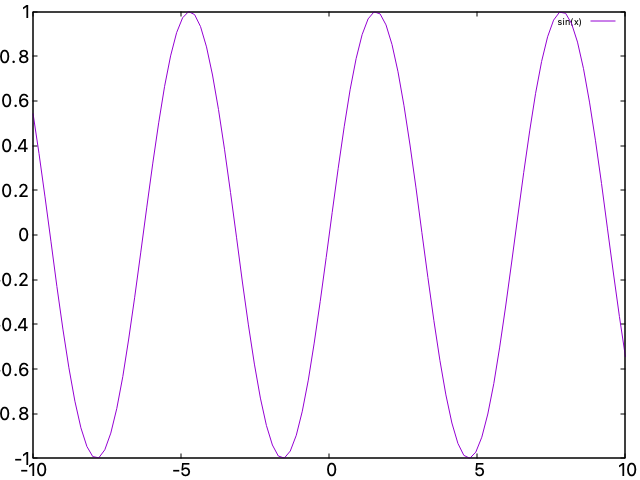
\includegraphics[width=0.7\textwidth]{fig1.png}
  \caption{\footnotesize This is an example on how to place a figure $0.85$ textwidth wide. 
  }
  \label{fig:single}
\end{figure}
%
%
\begin{figure}[!h]
  \centering
  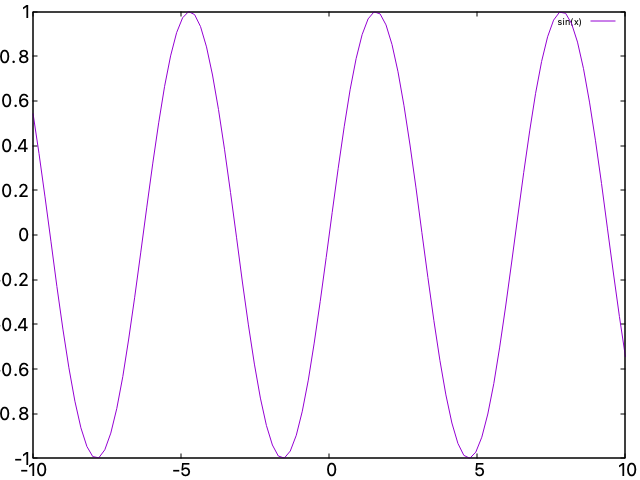
\includegraphics[width=0.45\textwidth]{fig1.png}%
  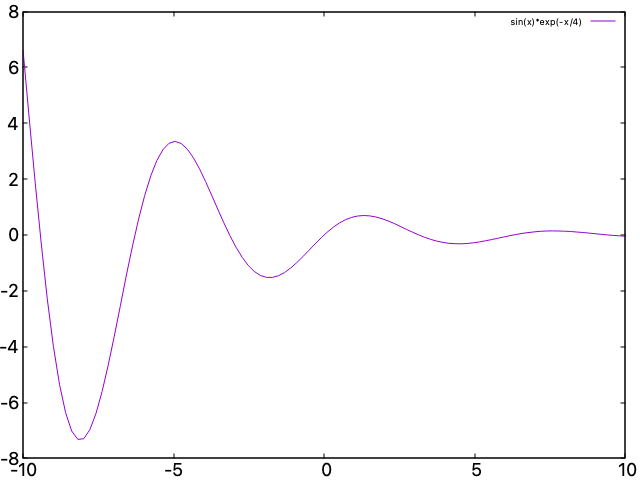
\includegraphics[width=0.45\textwidth]{fig2.png}
  \caption{\footnotesize How to place two figures side-by-side.
  Left: $\sin$ function; right: damped $\sin$ function.}
  \label{fig:double}
\end{figure}

%%%%%%%%%%%%%%%%%%%%%%%%%%%%%%%%%%%%%%%%%%%%%%%%%%%%%%%%%%%%%%%%%%%%%%%%
\clearpage   % The \clearpage command ends the current page and causes 
%              all figures and tables that have so far appeared in the input to be printed.
\section{Copy \& Paste your Code output}
%
%
%%%%%%%%%%%%%%%%%%%%%%%%%%%%%%%%%%%%%%%%%%%%%%%%%%%%%%%%%%%%%%%%%%%%%%%%

To report the output of the code, use can use the \texttt{verbatim} environment:
\begin{verbatim}
0.0   1.0   2.0
0.1   1.1   2.1
0.2   1.2   2.2
...

Copy your code output from terminal and paste it here ! 
...
\end{verbatim}


%%%%%%%%%%%%%%%%%%%%%%%%%%%%%%%%%%%%%%%%%%%%%%%%%%%%%%%%%%%%%%%%%%%%%%%%
\section{Inserting Code}
%
%
%%%%%%%%%%%%%%%%%%%%%%%%%%%%%%%%%%%%%%%%%%%%%%%%%%%%%%%%%%%%%%%%%%%%%%%%

Code can be inserted using the \texttt{lstlisting} environment included with the \texttt{listing} package included at the beginning of this document.
For instance:
\begin{verbatim}
  \begin{lstlisting}[language=C++]
      double i;
      for (i = ... ){
         ...
      }
      return;
  \end{lstlisting}

\end{verbatim}

An example of how it looks like is given below:

\begin{lstlisting}[language=C++]
  ...
  #include<iostream>
  #include<cmath>
  
  // Function prototype
  int    Factorial1(int);
  int    Factorial2(int);
  double Factorial3(int);
  double Factorial4(int);
  
  int main()
  {
    using namespace std;
    int number;
    double x = 1.0;
  
    cout << "Enter a number : ";
    cin  >> number;
  
    cout << number << "! = " << Factorial1(number) << endl;
    cout << number << "! = " << Factorial2(number) << endl;
    cout << number << "! = " << Factorial3(number) << endl;
    cout << number << "! = " << exp(Factorial4(number)) << endl;
  
    return(0);  
}
////////////////////////////////////////////////////////////////////////
int Factorial1 (int number)
//
//  Compute factorial using for loop
////////////////////////////////////////////////////////////////////////

{
  int ifact = 1;
  for (int i = 1; i <= number; i++) ifact = ifact*i; 
  return (ifact);
} 

\end{lstlisting}


If your code is long or you need to include more than one file, then a more efficient strategy is to use the \texttt{\textbackslash lstinputlisting[language=C++]\{fname.cpp\}} command.
This is show in the next example:

\lstinputlisting[language=C++]{template.cpp}

\end{document}

